\lecture{15}{21 April.}{}
\begin{eg}
    The \emph{friendship paradox} is the surprising fact that, in many social networks,
\textbf{your friends tend to have more friends than you do, on average}. This does not
mean every single friend is more popular than you. Instead, it means that when we sample
people by following friendship links, highly connected people are more likely to be seen,
because they appear in many people's friend lists.

\section*{A small graph intuition}

Consider the graph in \autoref{fig:friendship-paradox}. Each node is a person, and an
edge means a friendship. Node $C$ is a hub with degree $4$, while the other four nodes
have degree $1$.

\begin{figure}[H]
    \centering
    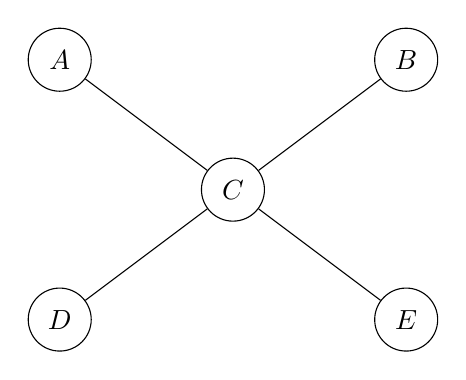
\begin{tikzpicture}[scale=1.1, every node/.style={circle, draw, minimum size=8mm}]
        \node (C) at (0,0) {$C$};
        \node (A) at (-2,1.5) {$A$};
        \node (B) at (2,1.5) {$B$};
        \node (D) at (-2,-1.5) {$D$};
        \node (E) at (2,-1.5) {$E$};

        \draw (C) -- (A);
        \draw (C) -- (B);
        \draw (C) -- (D);
        \draw (C) -- (E);
    \end{tikzpicture}
    \caption{A simple network where one person is much more connected than the others.}
    \label{fig:friendship-paradox}
\end{figure}

The average degree of all people in this network is
\[
\frac{1+1+4+1+1}{5} = \frac{8}{5} = 1.6.
\]
Now ask: if we pick a person and look at their friends, how many friends do those friends
typically have?

For $A$, the only friend is $C$, who has degree $4$. The same is true for $B$, $D$, and
$E$. Only $C$ sees low-degree neighbors. Because $C$ is listed as a friend by four
different people, $C$ gets counted over and over when we average over ``friends of
people.'' This pushes the average upward.

In fact, the average degree of a randomly chosen \emph{friend} in this graph is
\[
\frac{1^2 + 1^2 + 4^2 + 1^2 + 1^2}{1+1+4+1+1}
= \frac{20}{8} = 2.5,
\]
which is larger than $1.6$.

\section*{Why the paradox happens}

The key idea is \textbf{sampling bias}. People with many friends are more likely to show
up when we traverse edges, because each friendship gives them another chance to be
observed. In network terms, nodes with larger degree receive more weight.

If the degrees are $k_1, k_2, \dots, k_n$, then:
\[
\text{average degree of a person} = \frac{1}{n}\sum_{i=1}^n k_i,
\]
while the average degree of a person reached by following a random friendship edge is
\[
\frac{\sum_{i=1}^n k_i^2}{\sum_{i=1}^n k_i}.
\]

This second quantity is usually larger, because squaring gives extra weight to large
degrees. That is the mathematical reason the friendship paradox appears.

\section*{Takeaway}

The friendship paradox is not really about friendship in particular; it is a general fact
about networks. Whenever highly connected nodes are overrepresented in the way we sample,
our local view of the network makes others look more connected than the population average.
\end{eg}

\subsection{Normal Distribution}
We denote \(X \sim N(\mu , \sigma ^2)\) for some \(\mu \in \mathbb{R}\) (mean) and \(\sigma \in \mathbb{R} _{> 0}\) (standard deviation) for the normal distribution. 

\section*{What happens when the values change?}

\begin{itemize}[leftmargin=1.5em]
    \item \textbf{Larger $\mu$:} the whole curve moves to the \textbf{right}.
    \item \textbf{Smaller $\mu$:} the whole curve moves to the \textbf{left}.
    \item \textbf{Larger $\sigma$:} the curve becomes \textbf{wider and flatter}.
    \item \textbf{Smaller $\sigma$:} the curve becomes \textbf{narrower and taller}.
\end{itemize}

\begin{center}
\begin{tikzpicture}
\begin{groupplot}[
    group style={group size=2 by 1, horizontal sep=2cm},
    width=0.45\textwidth,
    height=0.34\textwidth,
    xmin=-6, xmax=6,
    ymin=0, ymax=0.85,
    samples=200,
    axis lines=left,
    xlabel={$x$},
    xlabel style={at={(axis description cs:1.04,-0.02)}, anchor=west},
    ylabel={density},
    legend style={draw=none, font=\small, at={(0.5,-0.36)}, anchor=north},
    every axis plot/.append style={thick}
]

\nextgroupplot[
    title={Effect of changing $\mu$},
]
\addplot[blue] {1/sqrt(2*pi)*exp(-((x+2)^2)/2)};
\addlegendentry{$\mu=-2,\ \sigma=1$}
\addplot[black] {1/sqrt(2*pi)*exp(-(x^2)/2)};
\addlegendentry{$\mu=0,\ \sigma=1$}
\addplot[red] {1/sqrt(2*pi)*exp(-((x-2)^2)/2)};
\addlegendentry{$\mu=2,\ \sigma=1$}

\nextgroupplot[
    title={Effect of changing $\sigma$},
]
\addplot[green!50!black] {1/(0.6*sqrt(2*pi))*exp(-(x^2)/(2*0.6^2))};
\addlegendentry{$\mu=0,\ \sigma=0.6$}
\addplot[black] {1/sqrt(2*pi)*exp(-(x^2)/2)};
\addlegendentry{$\mu=0,\ \sigma=1$}
\addplot[orange!90!black] {1/(1.8*sqrt(2*pi))*exp(-(x^2)/(2*1.8^2))};
\addlegendentry{$\mu=0,\ \sigma=1.8$}

\end{groupplot}
\end{tikzpicture}
\end{center}

\paragraph{pdf}
\[
    f_X(x) = \frac{1}{\sigma \sqrt{2 \pi}} e^{- \frac{(x - \mu )^2}{2 \sigma ^2}},
\]
which has \(f_X(x) > 0\) for all \(x\), so for any \(a < b\), \(\mathbb{P} (a \le x \le b) > 0\).    

\begin{claim}
    \[
        \int _{-\infty }^{\infty } f_X(x) \, \mathrm{d} x = 1.  
    \]
\end{claim}
\begin{explanation}
    Let \(I = \int _{-\infty }^{\infty } \frac{1}{\sigma \sqrt{2 \pi } } e^{- \frac{(x - \mu )^2}{2 \sigma ^2}} \, \mathrm{d} x\), and let \(z = \frac{x - \mu}{\sigma }\), so we have 
    \[
        I = \int _{-\infty }^{\infty} \frac{1}{\sigma \sqrt{2\pi } } e^{- \frac{z^2}{2}} \sigma \, \mathrm{d} z = \frac{1}{\sqrt{2\pi } } \int _{-\infty }^{\infty } e^{- \frac{z^2}{2}} \, \mathrm{d} z.  
    \]  
    Hence,
    \[
        I^2 = \left( \frac{1}{\sqrt{2\pi } } \int _{-\infty }^{\infty} e^{- \frac{z^2}{2}} \, \mathrm{d} z  \right) \left( \frac{1}{\sqrt{2\pi } } \int _{-\infty }^{\infty} e^{- \frac{y^2}{2}} \, \mathrm{d} y  \right) = \frac{1}{2\pi } \iint_{\mathbb{R} ^2} e^{- \frac{z^2 + y^2}{2}} \, \mathrm{d} z \, \mathrm{d} y.  
    \]
    Now we can substitute \(z = r \cos \theta \) and \(y = r \sin \theta \), and 
    \[
        \left\lVert \begin{pmatrix}
            \frac{\partial z}{\partial r}  & \frac{\partial z}{\partial \theta}   \\
            \frac{\partial y}{\partial r}  & \frac{\partial y}{\partial \theta}   \\
        \end{pmatrix} \right\rVert = \left\lVert \begin{pmatrix}
            \cos \theta  & -r \sin \theta   \\
            \sin \theta  & \cos \theta  \\
        \end{pmatrix} \right\rVert = r \cos ^2 \theta + r \sin ^2 \theta = r.  
    \]  
    Thus, \(\mathrm{d} z \, \mathrm{d} y = r \mathrm{d} r \, \mathrm{d} \theta    \). Hence,
    \[
        I^2 = \frac{1}{2\pi} \int _0^{2\pi } \int _{0} ^{\infty} e^{-\frac{(r\cos \theta )^2 + (r \sin \theta )^2}{2}} r \, \mathrm{d} r \, \mathrm{d} \theta = 1.   
    \]
    Hence, \(I = 1\). 
\end{explanation}

\begin{definition}
    We say \(N(0, 1)\) is the \emph{standard normal distribution}.
\end{definition}

Note that if \(Z \sim N(0, 1)\), then 
\[
    f_Z(z) = \frac{1}{\sqrt{2\pi}} e^{-\frac{z^2}{2}}.
\] 

\begin{claim}
    If \(X \sim N(\mu , \sigma ^2)\), then if \(Z = \frac{X - \mu}{\sigma}\), we have \(Z \sim N(0, 1)\).   
\end{claim}

\begin{explanation}
    \begin{align*}
        \mathbb{P} (Z \le z) &= \mathbb{P} \left( \frac{X - \mu}{\sigma} \le z \right) = \mathbb{P} (X \le \mu + z \sigma) = \int _{-\infty }^{\mu + z \sigma} \frac{1}{\sigma \sqrt{2 \pi} } e^{-\frac{(x - \mu )^2}{2 \sigma ^2}} \, \mathrm{d} x.  
    \end{align*}
    Now we change the variable, let \(t = \frac{x - \mu}{\sigma}\), i.e. \(x = \mu + t \sigma \), then we have 
    \[
        \mathbb{P} (Z \le z) = \int _{-\infty }^{\mu + z \sigma} \frac{1}{\sigma \sqrt{2 \pi} } e^{-\frac{(x - \mu )^2}{2 \sigma ^2}} \, \mathrm{d} x = \int _{-\infty }^z \frac{1}{\sqrt{2 \pi } } e^{-\frac{t^2}{2}} \, \mathrm{d} t = \mathbb{P} (N(0, 1) \le z).  
    \]  
\end{explanation}

\paragraph{Expectation}
Note that if \(Z \sim N(0, 1)\), then 
\begin{align*}
    \mathbb{E} [Z] &= \int _{-\infty }^{\infty } t f_Z(t) \, \mathrm{d} t = \frac{1}{\sqrt{2 \pi } } \int _{-\infty }^{\infty } t e^{-\frac{t^2}{2}} \, \mathrm{d} t = \frac{1}{\sqrt{2 \pi} } \left[ - e^{-\frac{t^2}{2}} \right]_{-\infty}^{\infty} = 0.   
\end{align*} 

Now if \(X \sim N(\mu , \sigma ^2)\), then \(Z = \frac{X - \mu}{\sigma}\), i.e. \(X = \mu + \sigma Z\), so 
\[
    \mathbb{E} [X] = \mu + \sigma \mathbb{E} [Z] = \mu .
\]   

\paragraph{Variance}
If \(Z \sim N(0, 1)\), then 
\[
    \mathbb{E} [Z^2] = \int _{-\infty }^{\infty } t^2 f_Z(t) \, \mathrm{d} t = \frac{1}{\sqrt{2 \pi } } \int _{-\infty }^{\infty } t \cdot \left[ t e^{-\frac{t^2}{2}} \right] \, \mathrm{d} t,   
\] 
and we can integration by parts: 
\begin{align*}
    \mathbb{E} [Z^2] &= \frac{1}{\sqrt{2 \pi}} \int _{-\infty }^{\infty } t \left( t e^{-\frac{t^2}{2}} \right) \, \mathrm{d} t = \frac{1}{\sqrt{2 \pi} } \left[ \left[ t(-e^{-\frac{t^2}{2}}) \right]_{-\infty }^{\infty } + \int _{-\infty }^{\infty } e^{-\frac{t^2}{2}} \, \mathrm{d} t  \right] = \int _{-\infty }^{\infty } \frac{1}{\sqrt{2 \pi} } e^{-\frac{t^2}{2}} \, \mathrm{d} t \\ &= \int _{-\infty }^{\infty} f_Z(t) \, \mathrm{d} t = 1.  
\end{align*}

Hence,
\[
    \Var(Z) = \mathbb{E} [Z^2] - \mathbb{E} [Z]^2 = 1 - 0 = 1.
\]

Thus, for \(X \sim N(\mu , \sigma ^2)\), we have \(Z = \frac{X - \mu}{\sigma }\), i.e. \(Z \sigma + \mu = X\). Hence,
\[
    \Var(X) = \mathbb{E} [(X - \mu)^2] = \mathbb{E} [(Z \sigma )^2] = \sigma ^2 \mathbb{E} [Z^2] = \sigma ^2.
\]   

\begin{eg}
    Suppose we have two envelops, one has \(\$ x\) and the other has \(\$ 2x\), and we choose one, and look inside, and we can choose whether or not to switch. What can we do to maximize our chances of getting more money?  
\end{eg}

\begin{explanation}
    Suppose the envelop we get has \(\$ y\), then there is \(50 \%\) of chance that \(y = x\) and the other has \(\$ 2y\), while there is \(50 \%\) of chance that \(y = 2x\) and the other has \(\frac{1}{2} y\). Thus,
    \[
        \mathbb{E} [\text{payout} ] = \frac{1}{2} (\$2y) + \frac{1}{2} (\$ \frac{1}{2} y) = \$ \frac{5}{4} y.
    \]       

    We can beat \(50 \%\) chance of getting the bigger envelop. The method is to let \(Z \sim N(0, 1)\) and sample \(z\) from \(Z\). If \(y < z\), then switch the envelop, and if \(y \ge z\), then keep the envelop. There are three cases:
    \begin{itemize}
        \item Case 1: \(z \le x\), always keep envelop, we have \(50 \%\) of winning. 
        \item Case 2: \(x < z \le 2x\), always get right right envelop, so we have \(100 \%\) of winning.  
        \item Case 3: \(2x < z\), always switch, so \(50\%\) of winning.    
    \end{itemize}  
    By the law of probability,
    \begin{align*}
        \mathbb{P} (\text{win} ) &= \mathbb{P} (\text{win} \mid z < x ) \mathbb{P} (z < x) + \mathbb{P} (\text{win} \mid x < z < 2x ) \mathbb{P} (x < z < 2x) + \mathbb{P} (\text{win} \mid 2x < z ) \mathbb{P} (2x < z) \\
        &= 50 \% \cdot \mathbb{P} (z \le x) + 100 \% \cdot \mathbb{P} (x < z \le 2x) + 50 \% \cdot \mathbb{P} (2x < z) \\
        &= 50 \% (1 - \mathbb{P} (x < z \le 2x)) + 100 \% \cdot \mathbb{P} (x < z \le 2x) \\
        &= 50\% + 50 \% \cdot \mathbb{P} (x < z \le 2x) > 50 \%.
    \end{align*}
\end{explanation}

Recall that if \(X \sim N(\mu , \sigma ^2)\), \(f_X(x) = \frac{1}{\sigma \sqrt{2 \pi } } e^{- \frac{(x - \mu )^2}{2 \sigma ^2}}\), then if we let \(Z = \frac{X - \mu}{\sigma }\), then \(Z \sim N(0, 1)\), we call \(Z\) to be the z-score. 

\paragraph{CDF}
\[
    F_Z(z) = \mathbb{P} (Z \le z) = \int _{-\infty }^z \frac{1}{\sqrt{2 \pi} } e^{- \frac{t^2}{2}} \, \mathrm{d} t \coloneqq \Phi (z), 
\]
which cannot be expressed by elementary functions.

\begin{remark}
    \hfill 
    \begin{itemize}
        \item [(i)] \(\mathbb{P} (a < Z \le b) = \mathbb{P} (Z \le b) - \mathbb{P} (Z \le a) = \Phi (b) - \Phi (a)\). 
        \item [(ii)] \(\mathbb{P} (Z > a) = 1 - \mathbb{P} (Z \le a) = 1 - \Phi (a)\). 
        \item [(iii)] By symmetry of this distribution,
        \[
            \Phi (z) = \mathbb{P} (Z \le z) = \mathbb{P} (Z \ge -z) = 1 - \mathbb{P} (Z \le -z) = 1 - \Phi (-z).
        \]
        Thus, it suffices to know \(\Phi (z)\) for \(z \ge 0\).   
        \begin{center}
        \begin{tikzpicture}
        \begin{axis}[
            width=12cm,
            height=7cm,
            domain=-3.6:3.6,
            samples=250,
            axis lines=middle,
            xlabel={$t$},
            ylabel={$f_Z(t)$},
            ymin=0,
            ymax=0.45,
            xmin=-3.6,
            xmax=3.6,
            xtick={-2,0,2},
            xticklabels={$-z$, $0$, $z$},
            ytick=\empty,
            clip=false
        ]
            \addplot[name path=normal, very thick, black] {1/sqrt(2*pi) * exp(-x^2/2)};
            \path[name path=axis] (axis cs:-3.6,0) -- (axis cs:3.6,0);

            \addplot[blue!35, draw=none] fill between[of=normal and axis, soft clip={domain=-3.6:-2}];
            \addplot[purple!45, draw=none] fill between[of=normal and axis, soft clip={domain=-2:2}];
            \addplot[red!35, draw=none] fill between[of=normal and axis, soft clip={domain=2:3.6}];

            \addplot[dashed] coordinates {(-2,0) (-2,{1/sqrt(2*pi) * exp(-(-2)^2/2)})};
            \addplot[dashed] coordinates {(2,0) (2,{1/sqrt(2*pi) * exp(-(2)^2/2)})};

            \node[blue!70!black] at (axis cs:-2.7,0.05) {left-only part};
            \node[purple!70!black] at (axis cs:0,0.18) {shared by both};
            \node[red!70!black] at (axis cs:2.7,0.05) {right-only part};
            \node[blue!70!black] at (axis cs:-1.9,0.29) {$\mathbb{P}(Z\le z)$};
            \node[red!70!black] at (axis cs:1.9,0.29) {$\mathbb{P}(Z\ge -z)$};
        \end{axis}
        \end{tikzpicture}
        \end{center}

        \item [(iv)] If \(X \sim N(\mu , \sigma ^2)\), 
        \[
            \mathbb{P} (X \le x) = \mathbb{P} \left( Z \le \frac{x - \mu}{\sigma} \right)  = \Phi \left( \frac{x - \mu}{\sigma} \right). 
        \]
    \end{itemize}
\end{remark}

\begin{eg}
    Transmitting binary data over a noise channel. If we send 1, then the receiver gets \(1 + X\); if we send 0, then the receiver gets \(X\), where \(X \sim N(0, 0.3^2)\). Our decoding algorithm is, when the receiver receives a number \(\ge 0.5\), then they will see it as 1, otherwise they see it as 0. Then, what is the probability of mistaking a bit?     
\end{eg}

\begin{explanation}
    Suppose the signal sent is \(S \in \left\{ 0, 1 \right\} \), then 
    \begin{align*}
        \mathbb{P} (\text{error}) &= \mathbb{P} (\text{error} \mid S = 0) \mathbb{P} (S = 0) + \mathbb{P} (\text{error} \mid S = 1) \mathbb{P} (S = 1) \\
        &= \mathbb{P} (X \ge 0.5) \mathbb{P} (S = 0) + \mathbb{P} (X < -0.5) \mathbb{P} (S = 1) \\
        &= \mathbb{P} (X < -0.5) \mathbb{P} (S = 0) + \mathbb{P} (X < -0.5) \mathbb{P} (S = 1) \quad (\text{by symmetry}) \\
        &= \mathbb{P} (X < -0.5) = \mathbb{P} \left( \frac{X - 0}{0.3} < \frac{-0.5}{0.3} \right) = \Phi \left( -1.67 \right).
    \end{align*}
    %fig

    \begin{figure}[H]
        \begin{center}
    \begin{tikzpicture}
        \begin{axis}[
            width=12cm,
            height=6.5cm,
            axis lines=middle,
            xmin=-1.1, xmax=2.1,
            ymin=0, ymax=1.55,
            xtick={0,0.5,1},
            xticklabels={$0$,$0.5$,$1$},
            ytick=\empty,
            enlargelimits=false,
            clip=false,
            domain=-1.1:2.1,
            samples=200,
            xlabel={$y$},
            every axis x label/.style={at={(current axis.right of origin)}, anchor=west},
        ]
            % left density: Y | S=0 ~ N(0, 0.3^2)
            \addplot[name path=A, very thick, draw=pink!70!black] {1/(0.3*sqrt(2*pi))*exp(-x^2/(2*0.3^2))};

            % right density: Y | S=1 ~ N(1, 0.3^2)
            \addplot[name path=B, very thick, draw=olive!70!black] {1/(0.3*sqrt(2*pi))*exp(-(x-1)^2/(2*0.3^2))};

            % x-axis path for shading
            \path[name path=axis] (axis cs:-1.1,0) -- (axis cs:2.1,0);

            % shaded error regions
            \addplot[pink!35, opacity=0.8] fill between[
                of=A and axis,
                soft clip={domain=0.5:2.1},
            ];
            \addplot[olive!35, opacity=0.8] fill between[
                of=B and axis,
                soft clip={domain=-1.1:0.5},
            ];

            % threshold line
            \addplot[dashed, gray] coordinates {(0.5,0) (0.5,1.45)};

            % labels
            \node[pink!70!black] at (axis cs:-0.08,1.38) {$S=0$};
            \node[olive!70!black] at (axis cs:1.08,1.38) {$S=1$};
            \node[gray!80] at (axis cs:0.58,1.48) {$y=0.5$};
        \end{axis}
    \end{tikzpicture}
    \end{center}
    \caption{Colored area represents misreading signal}
    \end{figure}
\end{explanation}